\subsection{Tổng quan về tổng hợp khuôn mặt}
Tổng hợp khuôn mặt là một bài toán đầy thách thức và hấp dẫn trong lĩnh vực đồ họa máy tính, bao gồm việc tổng hợp ảnh tĩnh cũng như hoạt hóa khuôn mặt. Các kỹ thuật tổng hợp không chỉ giới hạn trong việc tạo ra những hình ảnh chân thực cho công nghiệp điện ảnh hay trò chơi điện tử, mà còn đóng vai trò quan trọng trong các hệ thống tương tác người-máy và kỹ thuật talking head compression trong video hội thoại. Hơn nữa, những phương pháp này còn hỗ trợ đắc lực cho các bài toán nhận dạng khuôn mặt thông qua việc tạo ra các mẫu dữ liệu tổng hợp dưới nhiều góc độ và điều kiện chiếu sáng khác nhau.

\subsection{Các kỹ thuật nền tảng cốt lõi trong giáo trình}

\subsubsection{Mô hình hóa khuôn mặt}
Tóm tắt phương pháp dựng mô hình 3D từ chuỗi ảnh, hai hướng nhìn vuông góc hoặc một ảnh đơn.  


\subsubsection{Thay đổi điều kiện ánh sáng}

Trong vài năm gần đây, nhiều tiến bộ đáng kể đã đạt được trong lĩnh vực tạo ảnh chân dung chân thực dưới các điều kiện chiếu sáng tùy ý \cite{jiang2001face, wang2009shbmm, wen2003face, zhang2003face}. Một hướng tiếp cận phổ biến là kỹ thuật dựng hình ngược, cho phép tái tạo thuộc tính phản xạ bề mặt từ ảnh chụp để sau đó tổng hợp ảnh dưới môi trường sáng mới. Tuy nhiên, phương pháp này thường đòi hỏi thiết bị thu nhận chuyên dụng và chỉ phù hợp với các ứng dụng trong phòng thí nghiệm. Phần này trình bày hai kỹ thuật chính có tính ứng dụng cao hơn, bao gồm phương pháp ảnh tỷ lệ và phương pháp dựa trên hàm cơ sở Spherical Harmonics từ một ảnh đầu vào duy nhất.

\paragraph{Thay đổi ánh sáng bằng ảnh tỷ lệ.}
Riklin-Raviv và Shashua \cite{riklin2001quotient} đã đề xuất kỹ thuật ảnh tỷ lệ nhằm ánh xạ điều kiện chiếu sáng từ khuôn mặt này sang khuôn mặt khác. Ý tưởng cốt lõi dựa trên mô hình phản xạ Lambertian: với một điểm trên bề mặt khuôn mặt có albedo $\rho$ và pháp tuyến $\mathbf{n}$, cường độ sáng dưới hai điều kiện chiếu sáng lần lượt là $I = \rho E(\mathbf{n})$ và $I' = \rho E'(\mathbf{n})$, trong đó $E(\mathbf{n})$ và $E'(\mathbf{n})$ là irradiance tương ứng. Xét một khuôn mặt thứ hai có albedo $\rho_1$, cường độ sáng tương ứng là $I_1 = \rho_1 E(\mathbf{n})$ và $I'_1 = \rho_1 E'(\mathbf{n})$. Khi đó, ta có tỷ lệ bất biến theo albedo:
\begin{equation}
    \frac{I_1}{I} = \frac{I'_1}{I'},
\end{equation}
dẫn đến công thức tổng hợp ảnh khuôn mặt thứ hai dưới điều kiện chiếu sáng mới:
\begin{equation}
\label{eq:ratio_image}
    I'_1 = I' \cdot \frac{I_1}{I}.
\end{equation}
Phương trình \eqref{eq:ratio_image} cho thấy rằng nếu ta có sẵn ảnh của một người dưới mọi điều kiện chiếu sáng cùng ảnh của người thứ hai dưới một điều kiện bất kỳ, ta hoàn toàn có thể tổng hợp ảnh của người thứ hai dưới tất cả các điều kiện chiếu sáng còn lại. Trong trường hợp không biết trước điều kiện chiếu sáng của ảnh đầu vào, Riklin-Raviv và Shashua \cite{riklin2001quotient} đề xuất sử dụng một cơ sở dữ liệu ảnh của nhiều người dưới nhiều điều kiện sáng khác nhau. Nếu albedo của khuôn mặt mới nằm trong khoảng bao quát hợp lý của cơ sở dữ liệu, hệ thống có thể suy ra điều kiện chiếu sáng gốc mà không cần thông tin bổ sung.

\paragraph{Thay đổi ánh sáng từ một ảnh đơn.}
Một hướng tiếp cận mạnh mẽ hơn cho phép thay đổi ánh sáng mà không cần cơ sở dữ liệu đã được Wen et al. \cite{wen2003face} phát triển. Xuất phát từ một ảnh khuôn mặt duy nhất, phương pháp này tính toán một bản đồ bức xạ đặc biệt bằng cách khai triển hàm irradiance theo các hàm cơ sở Spherical Harmonics. Cụ thể, irradiance tại pháp tuyến $\mathbf{n}$ được xấp xỉ bởi tổ hợp tuyến tính của chín hàm cơ sở Spherical Harmonics bậc thấp:
\begin{equation}
\label{eq:irradiance_sh}
    E(\mathbf{n}) \approx \sum_{\substack{l \le 2 \\ -l \le m \le l}} \hat{A}_l L_{lm} Y_{lm}(\mathbf{n}),
\end{equation}
trong đó $\hat{A}_l$ là hệ số lọc tần phản xạ, $L_{lm}$ là hệ số chiếu sáng và $Y_{lm}(\mathbf{n})$ là các hàm Spherical Harmonics.

Đồng thời, hàm albedo $\rho(\mathbf{n})$ cũng được khai triển dưới dạng:
\begin{equation}
    \rho(\mathbf{n}) = \rho_{00} + \Psi(\mathbf{n}),
\end{equation}
trong đó $\rho_{00}$ là thành phần hằng số (albedo trung bình) và $\Psi(\mathbf{n})$ chứa các thành phần bậc cao hơn. Wen et al. \cite{wen2003face} lập luận rằng da mặt con người gần như thỏa mãn giả thiết $\Psi(\mathbf{n})$ không chứa các thành phần tần số thấp bậc $l = 1, 2, 3, 4$. Nhờ tính trực giao của các hàm Spherical Harmonics, chín hệ số bậc $l \le 2$ ước lượng từ tích $\rho(\mathbf{n})E(\mathbf{n})$ bằng phương pháp bình phương tối thiểu tuyến tính chính là $\rho_{00}\hat{A}_l L_{lm}$, cho phép thu được bản đồ bức xạ với hệ số phản xạ bằng albedo trung bình.

Sử dụng hình học khuôn mặt 3D tổng quát, Wen et al. \cite{wen2003face} thiết lập hệ phương trình:
\begin{equation}
\label{eq:sh_system}
    I(\mathbf{n}) = \sum_{\substack{l \le 2 \\ -l \le m \le l}} x_{lm} Y_{lm}(\mathbf{n}),
\end{equation}
và giải hệ phương trình bình phương tối thiểu tuyến tính cho chín ẩn số $x_{lm}$ để thu được bản đồ bức xạ đặc biệt.

Từ bản đồ bức xạ thu được, việc thay đổi ánh sáng khuôn mặt được thực hiện thông qua kỹ thuật ảnh tỷ lệ. Khi khuôn mặt xoay trong môi trường sáng cố định, pháp tuyến tại mỗi điểm chuyển từ $\mathbf{n}$ sang $\mathbf{n}'$, cường độ sáng mới được tính theo:
\begin{equation}
\label{eq:relight_ratio}
    I'_f = I_f \cdot \frac{I_s(\mathbf{n}')}{I_s(\mathbf{n})},
\end{equation}
trong đó $I_f$ là cường độ sáng gốc trên khuôn mặt, $I_s(\mathbf{n})$ và $I_s(\mathbf{n}')$ lần lượt là cường độ trên bản đồ bức xạ tại pháp tuyến cũ và mới. Hình \ref{fig:relight_comparison} minh họa kết quả thay đổi ánh sáng: ảnh tổng hợp ở hàng dưới khớp tốt với ảnh thực tế ở hàng trên, chỉ có sai khác nhỏ ở các vùng phản xạ gương do da mặt có tính non-Lambertian ở các góc chiếu sáng lớn \cite{marschner1999skin}.

\begin{figure}[htbp]
    \centering
    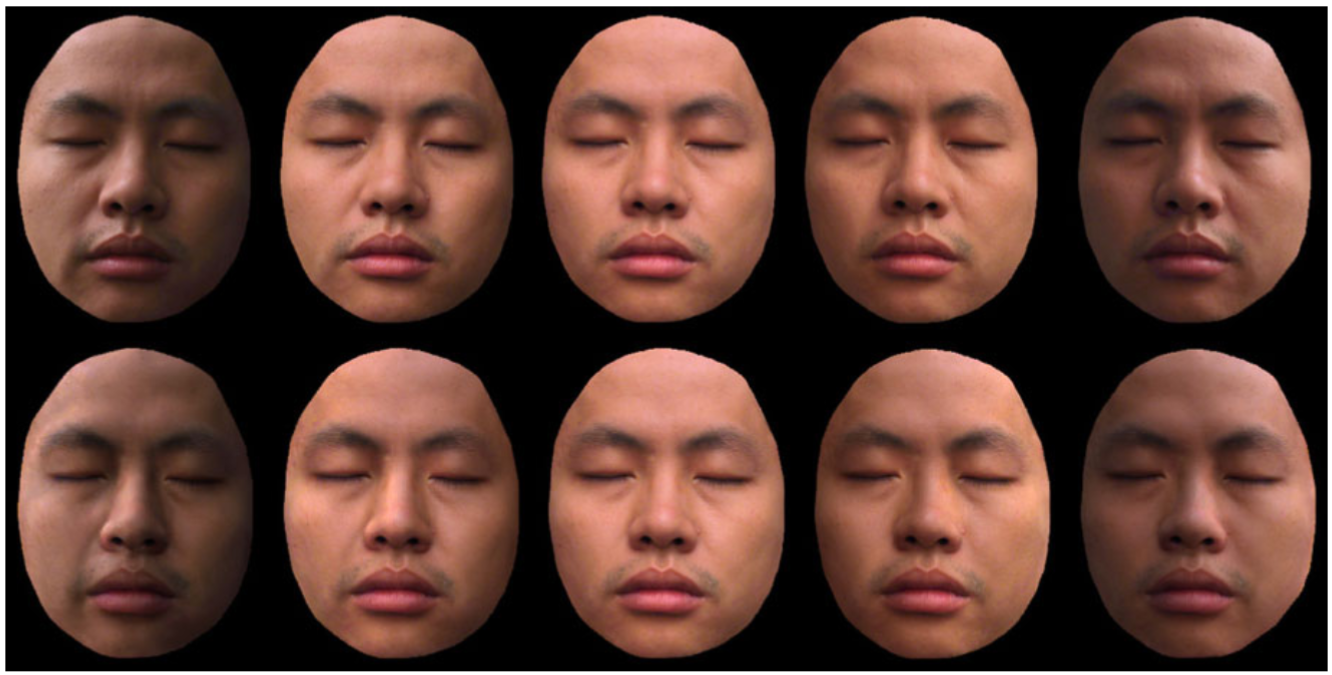
\includegraphics[width=0.85\textwidth]{img/Fig.20.7.png}
    \caption{So sánh kết quả tổng hợp và ảnh thực tế. Hàng trên là ảnh thực tế, hàng dưới là ảnh tổng hợp, ảnh giữa hàng dưới là ảnh đầu vào \cite{wen2003face}.}
    \label{fig:relight_comparison}
\end{figure}

Ngoài ra, phương pháp này còn cho phép chỉnh sửa chiếu sáng bằng cách điều chỉnh trực tiếp các hệ số Spherical Harmonics đã ước lượng. Với mỗi bộ hệ số mới, kỹ thuật ảnh tỷ lệ trong phương trình \eqref{eq:relight_ratio} được áp dụng để tạo ảnh khuôn mặt dưới điều kiện sáng tương ứng. Hình \ref{fig:lighting_editing} trình bày bốn ví dụ chỉnh sửa chiếu sáng: thêm bóng đổ lên một bên mặt, thay đổi sắc độ màu ánh sáng theo hướng, di chuyển vùng sáng chính từ bên này sang bên kia, và kết hợp cả bóng đổ lẫn thay đổi màu sắc. Khả năng tạo dữ liệu huấn luyện đa dạng về chiếu sáng từ phương pháp này có giá trị lớn cho các bài toán phát hiện và nhận dạng khuôn mặt.

\begin{figure}[htbp]
    \centering
    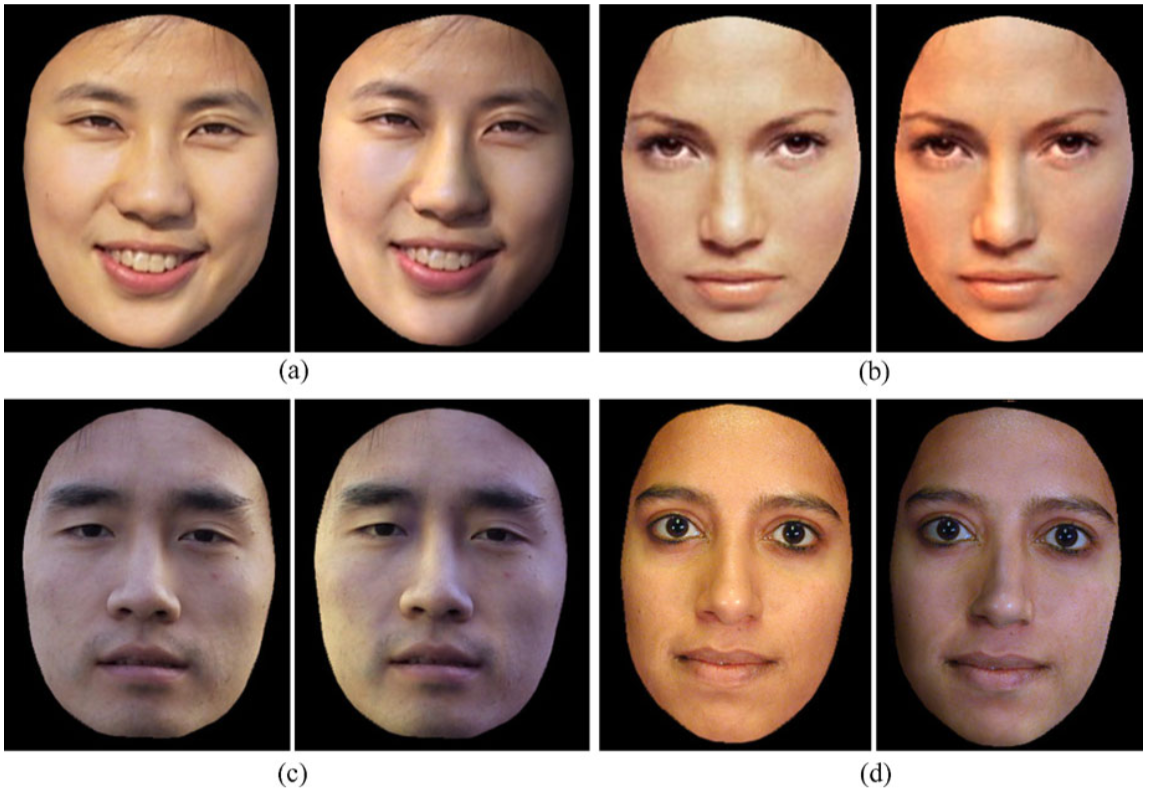
\includegraphics[width=0.85\textwidth]{img/Fig.20.8.png}
    \caption{Chỉnh sửa ánh sáng bằng cách thay đổi hệ số Spherical Harmonics của bản đồ bức xạ. Ảnh bên trái mỗi cặp là ảnh đầu vào, ảnh bên phải là kết quả sau khi chỉnh sửa ánh sáng \cite{wen2003face}.}
    \label{fig:lighting_editing}
\end{figure}

\paragraph{Ứng dụng trong nhận dạng khuôn mặt dưới điều kiện chiếu sáng thay đổi.}
Qing et al. \cite{qing2004face} đã ứng dụng kỹ thuật thay đổi ánh sáng vừa trình bày vào bài toán nhận dạng khuôn mặt dưới các môi trường chiếu sáng khác nhau. Với mỗi ảnh khuôn mặt đầu vào dưới chiếu sáng không xác định, phương pháp này trước tiên tạo ảnh mới dưới chiếu sáng chuẩn hóa, tức là chỉ giữ lại thành phần hằng số $x_{00}$ trong khai triển Spherical Harmonics ở phương trình \eqref{eq:sh_system} và đặt các hệ số còn lại bằng không. Kỹ thuật ảnh tỷ lệ trong phương trình \eqref{eq:relight_ratio} sau đó được sử dụng để sinh ảnh dưới chiếu sáng chuẩn hóa. Quá trình đối sánh ảnh được thực hiện trên các ảnh đã chuẩn hóa chiếu sáng. Thực nghiệm trên cơ sở dữ liệu PIE \cite{sim2003pie} cho thấy tỷ lệ nhận dạng được cải thiện đáng kể sau khi áp dụng kỹ thuật thay đổi ánh sáng.


\subsubsection{Tổng hợp biểu cảm khuôn mặt}

Tổng hợp biểu cảm khuôn mặt là một chủ đề nghiên cứu sôi nổi nhằm tạo ra các hình ảnh biểu cảm chân thực. Các kỹ thuật tổng hợp biểu cảm khuôn mặt nhìn chung có thể được chia thành ba hướng tiếp cận chính: tổng hợp dựa trên vật lý, tổng hợp dựa trên biến hình (morphing) và ánh xạ biểu cảm.

\paragraph{Tổng hợp biểu cảm dựa trên vật lý.}
Một trong những hướng tiếp cận ban đầu dựa trên mô hình vật lý là sử dụng mô hình khối lượng và lò xo (mass and spring) để mô phỏng da \cite{badler19813d}. Trong mô hình này, một tập hợp các cơ được gắn vào các đỉnh của lưới da; khi cơ co lại sẽ tạo ra lực tác động làm biến dạng lưới da. Để cải thiện khả năng mô phỏng, Waters \cite{waters1987muscle} đã giới thiệu các loại cơ vòng và cơ tuyến tính, đồng thời định nghĩa vùng ảnh hưởng cho mỗi cơ để giảm dần tác động khi càng xa điểm gắn. Kế tiếp, Terzopoulos và Waters \cite{terzopoulos1990physically} mở rộng mô hình này với cấu trúc mô khuôn mặt ba lớp, bổ sung thêm lớp mô mỡ giữa cơ và da để cung cấp khả năng kiểm soát biến dạng da tinh tế hơn. Mặc dù vậy, hạn chế chung của các phương pháp dựa trên vật lý là khó tạo ra các biểu cảm tự nhiên, do các chuyển động vi mô của da như nếp nhăn rất khó mô phỏng chỉ bằng cơ chế khối lượng và lò xo.

\paragraph{Tổng hợp biểu cảm dựa trên biến hình.}
Kỹ thuật biến hình (morphing) hay nội suy (interpolation) tổng hợp các biểu cảm mới bằng cách pha trộn một tập hợp các biểu cảm mẫu 2D hoặc 3D. Từ những công trình tiên phong của Parke \cite{parke1972computer}, phương pháp này đã được ứng dụng rộng rãi. Pighin và cộng sự \cite{pighin1998synthesizing} áp dụng kỹ thuật biến hình trên cả lưới 3D và ảnh kết cấu (texture) để tạo ra các biểu cảm 3D chân thực. Họ sử dụng tổ hợp tuyến tính lồi của các ví dụ biểu cảm và cho phép người dùng chỉ định các vùng hoạt động riêng biệt nhằm tăng cường kiểm soát cục bộ. Tuy nhiên, phương pháp này bị giới hạn ở không gian biểu cảm mà các mẫu hiện có thể sinh ra. Việc phân chia các vùng cục bộ không hợp lý có thể dẫn đến hiện tượng bóng mờ tại ranh giới, dù một số phương pháp phân chia vùng tự động đã được đề xuất để giải quyết vấn đề này \cite{joshi2003learning}.

\paragraph{Ánh xạ biểu cảm.}
Ánh xạ biểu cảm, hay hoạt họa điều khiển bằng diễn xuất (performance-driven animation), là kỹ thuật phổ biến để tạo ra các biểu cảm chân thực. Dựa trên ảnh chụp khuôn mặt trung lập và khuôn mặt mang biểu cảm, vị trí các đặc trưng khuôn mặt (mặt, lông mày, miệng, ...) được xác định, sau đó vector khác biệt của các điểm này được cộng vào vị trí đặc trưng của khuôn mặt đích thông qua kỹ thuật biến dạng hình ảnh được điều khiển bằng hình học.

Để tái tạo chi tiết biểu cảm một cách tự nhiên, Liu và cộng sự \cite{liu2001expressive} đề xuất sử dụng ảnh tỉ số biểu cảm (Expression Ratio Image - ERI). Kỹ thuật này trích xuất sự thay đổi chiếu sáng do biến dạng da một cách độc lập với màu da, từ đó áp dụng lên khuôn mặt khác để tái tạo các chi tiết vi mô. Giả sử $I_a$ là ảnh trung lập của người A và $I'_a$ là ảnh biểu cảm tương ứng. Tỉ số $\frac{I'_a}{I_a}$ phản ánh sự thay đổi ánh sáng do thay đổi pháp tuyến bề mặt. Tỉ số này sau đó được nhân trực tiếp vào ảnh khuôn mặt trung lập $I_b$ của người B để sinh ra ảnh biểu cảm đích $I'_b$:

\begin{equation}
    I'_b = I_b \frac{I'_a}{I_a}.
\end{equation}

Hình \ref{fig:eri_expression} minh họa ảnh tỉ số biểu cảm, trong khi Hình \ref{fig:mapping_thinking} cho thấy kết quả ánh xạ chi tiết biểu cảm sinh động hơn so với kỹ thuật biến dạng hình học truyền thống. Hình \ref{fig:mapping_mona_lisa} cho thấy kết quả ánh xạ biểu cảm cười (Hình \ref{fig:smile_expression}) lên khuôn mặt nàng Mona Lisa. Hình \ref{fig:mapping_statues} hiển thị kết quả ánh xạ biểu cảm cười lên hai bức tượng.

\begin{figure}[!htbp]
    \centering
    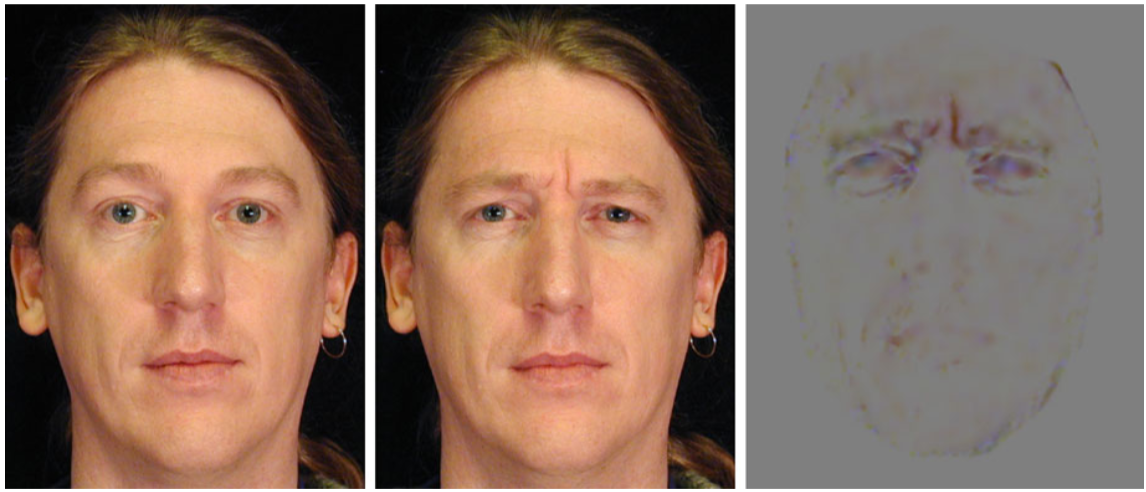
\includegraphics[width=0.65\textwidth]{img/Fig.20.9.png}
    \caption{Ảnh tỉ số biểu cảm (ERI) với từ trái qua phải là ảnh khuôn mặt trung lập, ảnh khuôn mặt có biểu cảm và ERI tương ứng \cite{liu2001expressive}.}
    \label{fig:eri_expression}
\end{figure}

\begin{figure}[!htbp]
    \centering
    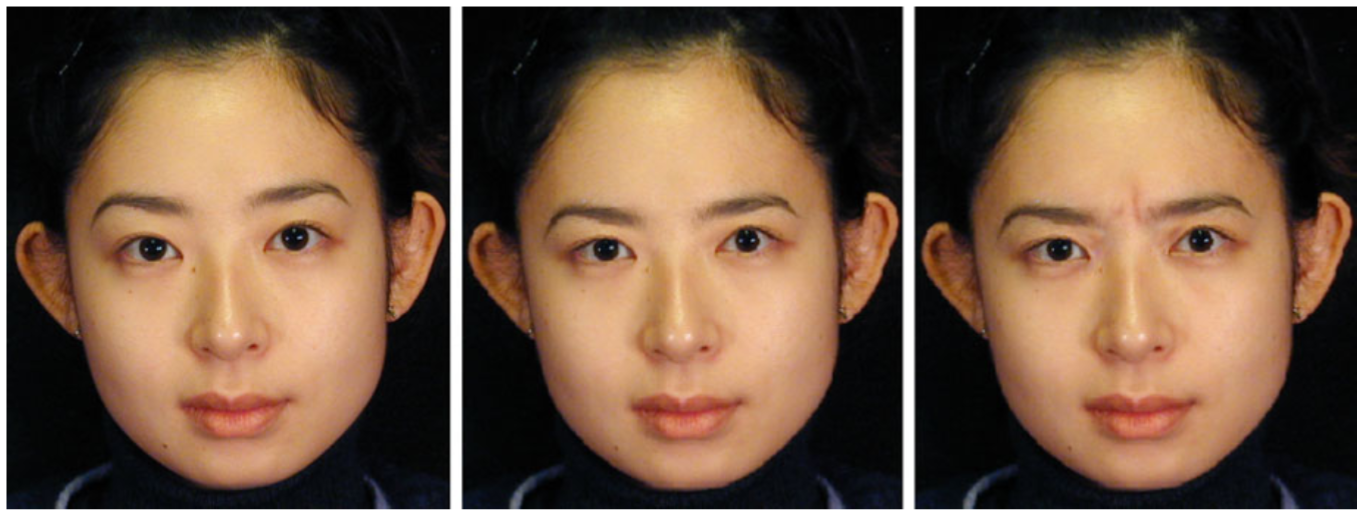
\includegraphics[width=0.75\textwidth]{img/Fig.20.10.png}
    \caption{Kết quả ánh xạ biểu cảm suy nghĩ bằng kỹ thuật biến dạng hình học (giữa) và kỹ thuật ERI (phải) \cite{liu2001expressive}.}
    \label{fig:mapping_thinking}
\end{figure}

\begin{figure}[!htbp]
    \centering
    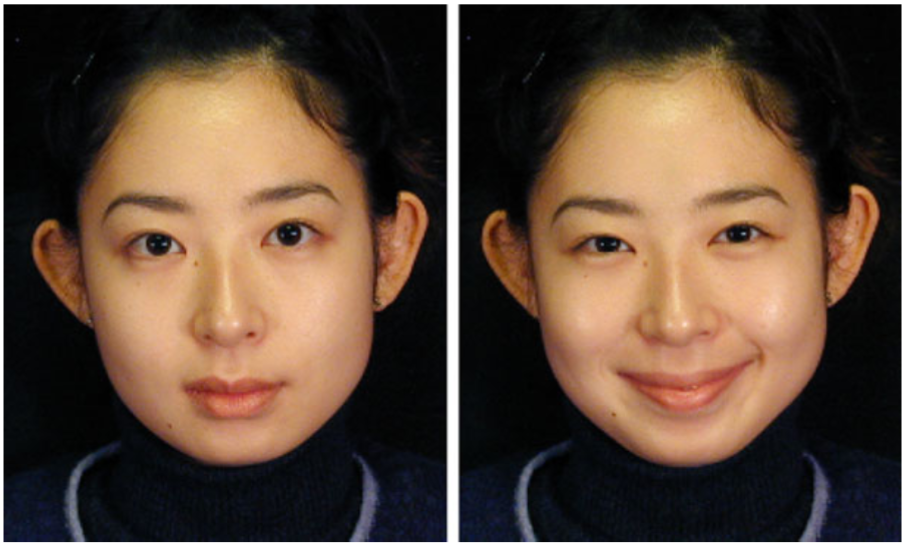
\includegraphics[width=0.4\textwidth]{img/Fig.20.11.png}
    \caption{Biểu cảm cười được dùng để ánh xạ lên khuôn mặt người khác.}
    \label{fig:smile_expression}
\end{figure}

\begin{figure}[!htbp]
    \centering
    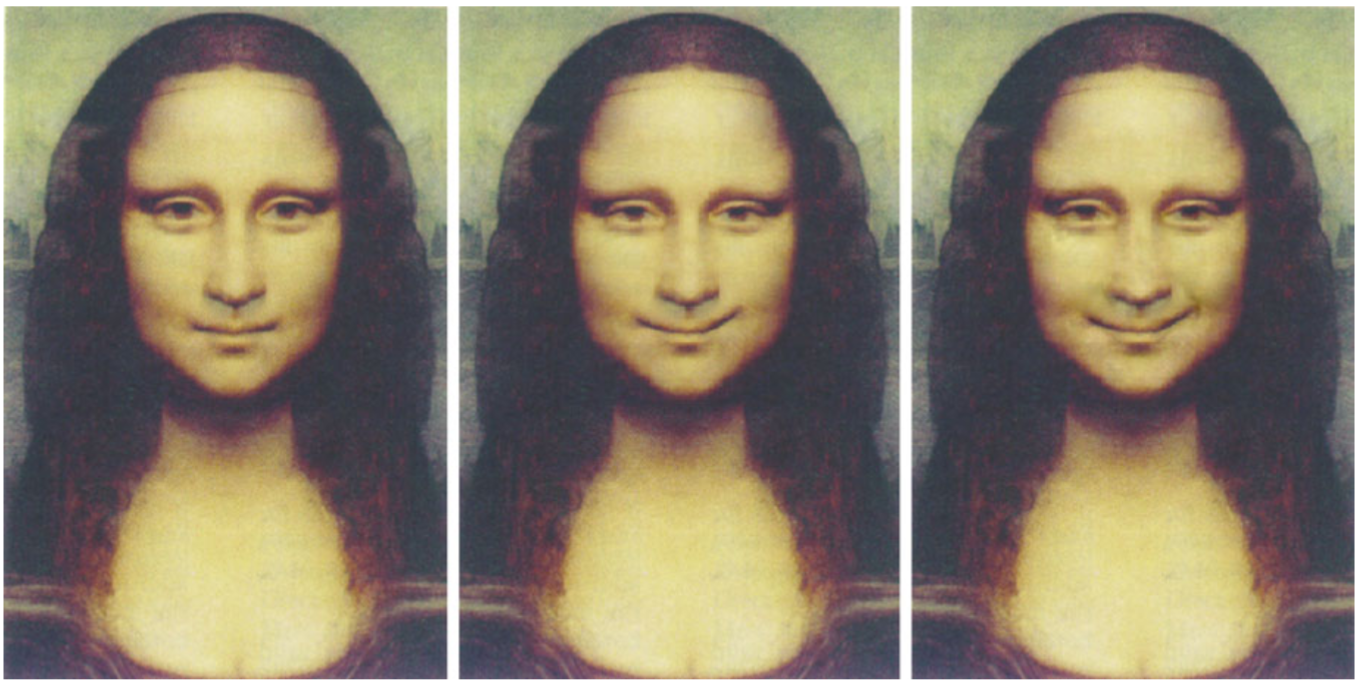
\includegraphics[width=0.85\textwidth]{img/Fig.20.12.png}
    \caption{Kết quả ánh xạ biểu cảm cười lên khuôn mặt nàng Mona Lisa. Trái: khuôn mặt trung lập. Giữa: kết quả từ biến dạng hình học. Phải: kết quả từ ERI \cite{liu2001expressive}.}
    \label{fig:mapping_mona_lisa}
\end{figure}

\begin{figure}[!htbp]
    \centering
    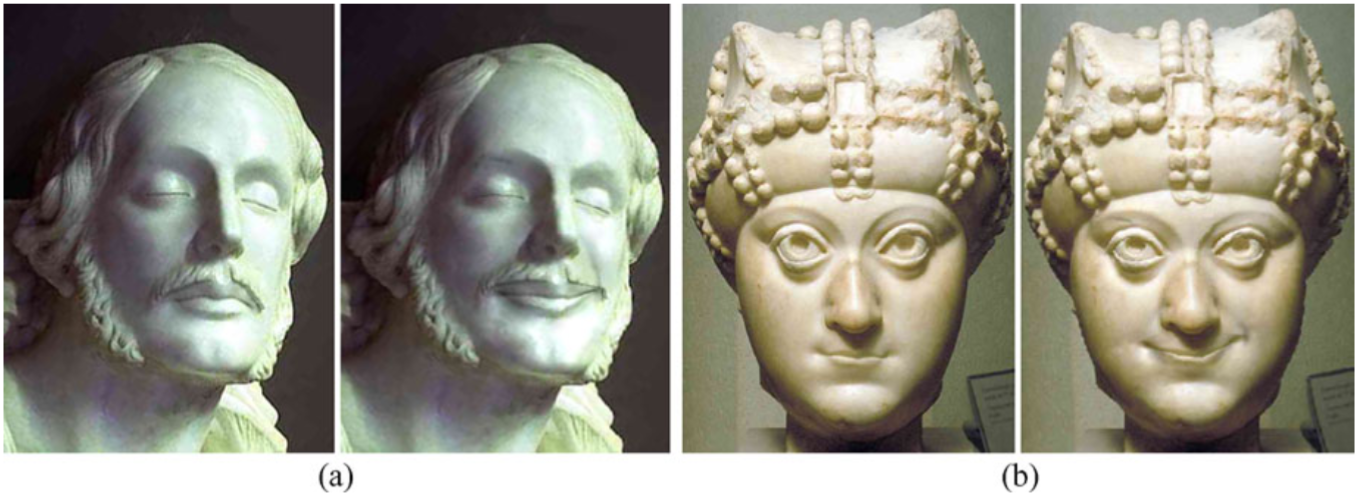
\includegraphics[width=0.85\textwidth]{img/Fig.20.13.png}
    \caption{Kết quả ánh xạ biểu cảm lên các bức tượng. (a) Trái: bức tượng gốc. Phải: kết quả từ ERI. (b) Trái: một bức tượng khác. Phải: kết quả từ ERI \cite{liu2001expressive}.}
    \label{fig:mapping_statues}
\end{figure}

Nhược điểm của kỹ thuật ERI là yêu cầu phải có ảnh tỉ số biểu cảm từ người diễn xuất. Để khắc phục điều này, Zhang và cộng sự \cite{zhang2003geometry} đề xuất hệ thống tổng hợp biểu cảm điều khiển bằng hình học, chỉ yêu cầu chuyển động của các điểm đặc trưng. Hệ thống giả định rằng mọi biểu cảm đều nằm trong không gian tổ hợp lồi của các ví dụ mẫu $E_i = (G_i, I_i)$:

\begin{equation}
    H(E_0, \dots, E_m) = \left\{ \left( \sum_{i=0}^{m} c_i G_i, \sum_{i=0}^{m} c_i I_i \right) \;\middle|\; \sum_{i=0}^{m} c_i = 1, c_i \ge 0 \right\}.
\end{equation}

Bằng cách chiếu thành phần hình học của biểu cảm mới vào bao lồi của các ví dụ, các hệ số $c_i$ được tối ưu hóa và sử dụng để tổng hợp thành phần kết cấu tương ứng. Để hỗ trợ không gian biểu cảm đa dạng, khuôn mặt được chia thành nhiều vùng xử lý độc lập như Hình \ref{fig:geometry_driven_synthesis}. Hệ thống còn tích hợp thuật toán lan truyền chuyển động dựa trên phân tích thành phần chính phân cấp nhằm tự động hoàn thiện chuyển động của toàn bộ khuôn mặt từ một số ít điểm đặc trưng cơ bản.

\begin{figure}[!htbp]
    \centering
    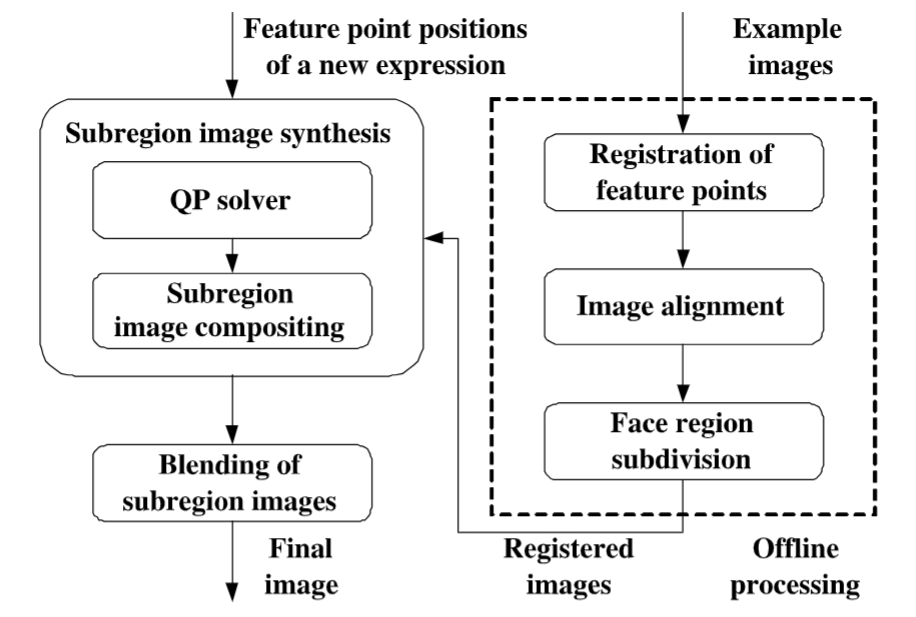
\includegraphics[width=0.6\textwidth]{img/Fig.20.14.png}
    \caption{Tổng quan kiến trúc hệ thống tổng hợp biểu cảm điều khiển bằng hình học \cite{zhang2003geometry}.}
    \label{fig:geometry_driven_synthesis}
\end{figure}


\subsubsection{Thảo luận và Định hướng}
Những kỹ thuật truyền thống đã tạo ra nền móng vững chắc cho việc mô hình hóa, chiếu sáng và tổng hợp biểu cảm. Tuy nhiên, thách thức lớn vẫn nằm ở việc tự động hóa và vượt qua các giới hạn nội suy cục bộ. Các phương pháp dựa trên hình học hoặc vật lý khó thể hiện sự phong phú vô tận của sắc thái con người nếu thiếu dữ liệu đầu vào dày đặc, mở ra không gian cho các phương pháp sinh hình ảnh mang tính khái quát cao hơn.
